\section{Example: San Miguel}
\label{sec:example}

Although purely theoretical, we can walk through a potential execution
of our algorithm and draw some conclusions on how it may perform.
Using the San Miguel data set
% RRL: citation?
and assuming we decompose the domain into 27 equal parts, we get the
distribution shown in Figure~\ref{fig:decomposition}. This will be the
cost of communicating the initial datasets to the nodes where
execution will take place. We will incur these costs again if data
needs to be moved once the algorithm starts executing.

\begin{figure}[!htb]
  \centering
  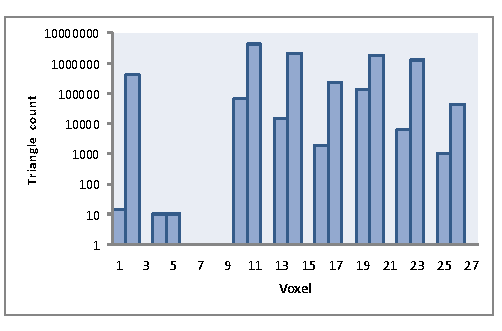
\includegraphics[width=0.5\textwidth]{drawings/DataDistribution.pdf}
  \caption{San Miguel Data Decomposition}
  \label{fig:decomposition}
\end{figure}

If we consider a machine with 8 cores, we might hope to get a distribution such as that shown in Figure~\ref{fig:machines}.   This roughly distributes the data evenly putting an emphasis on positioning neighbors on the same cores.  Depending on the lights in the scene, we also have to consider the cost of distributing them, building the light mesh, and sending the light mesh data to each node.  For this example I am assuming the costs associated with the lighting is negligible next to the cost of distributed the data in the scene. 

>>> RESUME

\begin{figure}[!htb]
  \centering
  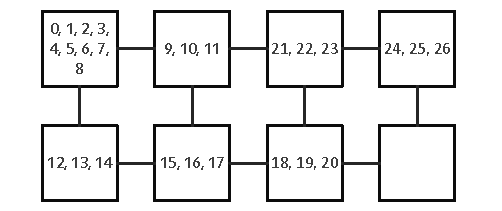
\includegraphics[width=0.5\textwidth]{drawings/NodeDistribution.pdf}
  \caption{Sample Data Distribution}
  \label{fig:machines}
\end{figure} 

Once the algorithm begins execution we can assume a worst case of 3 ray steps being necessary to trace rays from the camera through the scene.  This means each voxel will need to communicate with its neighbors a maximum of 3 times. Some of this communication will be within a node, some will be between nodes.  The cost of this communication needs to be factored into our estimates for total time to trace a given scene.  Acquiring accurate estimates for this equation will be the focus of our future work as exascale systems do not yet exist.  

%%% Local Variables: 
%%% mode: latex
%%% TeX-master: "main"
%%% End: 
